\documentclass[12pt,a4page]{article}

% AMS packages:
\usepackage{amsfonts}
\usepackage{amssymb}
\usepackage{amsmath}
\usepackage{amsthm}
\usepackage{epsfig}
\usepackage{graphicx}
\usepackage{natbib}		% citet, citep
\usepackage{textcomp}
\usepackage{booktabs}
\usepackage{multirow}
\usepackage{fullpage}
\usepackage{color}
\usepackage{graphicx}
% for table
\usepackage{tabularx}

% for algorithm
\usepackage{algorithm}
\usepackage{algpseudocode}
\usepackage{amsmath}
\usepackage{graphics}
\usepackage{epsfig}

\renewcommand{\baselinestretch}{1.5}

% Theorems
%-----------------------------------------------------------------
\newtheorem{thm}{Theorem}[section]
\newtheorem{cor}[thm]{Corollary}
\newtheorem{lem}[thm]{Lemma}
\newtheorem{prop}[thm]{Proposition}
\theoremstyle{definition}
\newtheorem{defn}[thm]{Definition}
\theoremstyle{remark}
\newtheorem{rem}[thm]{Remark}

% Shortcuts.
% One can define new commands to shorten frequently used
% constructions. As an example, this defines the R and Z used
% for the real and integer numbers.
%-----------------------------------------------------------------
\def\RR{\mathbb{R}}
\def\ZZ{\mathbb{Z}}

% Similarly, one can define commands that take arguments. In this
% example we define a command for the absolute value.
% -----------------------------------------------------------------
\newcommand{\abs}[1]{\left\vert#1\right\vert}

% Operators
% New operators must defined as such to have them typeset
% correctly. As an example we define the Jacobian:
% -----------------------------------------------------------------
\DeclareMathOperator{\Jac}{Jac}

%-----------------------------------------------------------------
\title{ Optimization for a joint predictive maintenance and job scheduling problem in manufacturing industry }

\iffalse
\author{Ling-Chieh Kung, Zih-Yun Liao, Wen-Yu Kung, Kai-Hsiang Huang}
\fi
\date{}

\renewcommand{\baselinestretch}{1.5}

\begin{document}

\maketitle

\iffalse
\abstract{This is a simple template for an article written in \LaTeX.}
\fi
\section{Introduction}

Maintenance is an integral component of operating manufacturing equipment. There are a lot of past studies in different maintenance models and policies \citep{wang2002}. Most types of maintenance fall under two main categories: preventive and corrective maintenance \citep{mobley2002}. \textit{Corrective maintenance}, also known as run-to-failure maintenance,  is a reactive management technique which is initiated only when a machine breaks down.  On the other hand, \textit{preventive maintenance} is based on elapsed time or hours of operation. \textit{Predictive maintenance} is one kind of condition-driven preventive maintenance, which determines the maintenance schedule of each machine by monitoring the mechanical condition, system efficiency, and other indicators. In contrast to the traditional preventive maintenance, which is only conducted on the same schedule every cycle, predictive maintenance is conducted as needed, drawing on real-time collection and analysis of machine operation data to identify issues at the nascent stage before they may interrupt production. Predictive maintenance provides a flexible way to determine maintenance schedule and often involves prognostic and health management (PHM), which is more complex and may require new equipment and technology in order to collect and share data with a centralized system.

\iffalse
PHM is an emerging engineering discipline which aims to diagnose and predict the future performance of a component by assessing the degradation of a system from its normal operating conditions. Due to the unexpected events such as equipment failures that can lead to additional costs and are difficult to manage, the profitability of a company largely depends on their maintenance schedule. PHM is now an important issue and helps people implement a better predictive maintenance schedule, which improves machine availability, efficiency, and product quality during the production process.
\fi

Taiwan is one of the world's largest providers in the electronics manufacturing industry. The production process in the electronics manufacturing industry strongly relies on the availability of machines and usually spends a high cost on machine maintenance. Although machines nowaday are more advanced and reliable than those in the past, they are still subject to deterioration because of ageing and requires maintenance. The planned production schedule are thus often influenced consequently. Therefore, maintenance plays an important role in production scheduling problems, especially in the electronics manufacturing industry.

However, since predictive maintenance is usually complex and the maintenance effect is not well predicted, maintenance and production issues are usually considered separately. Most of the studies do not simultaneously take scheduling and maintenance planning decisions into account, which means the production quality may be overestimated and the production cost may be underestimated. We propose a general model which considers both production scheduling and maintenance planning decisions, and the objective is to minimize the total cost.

In our study, we consider a production scheduling problem with irregular predictive maintenance. There are products with different demand levels ready to be processed. Each product must be processed from various stations to fulfill certain demand. A decision maker will decide the production and the maintenance schedule in each machine to minimize the total cost of the production. Maintenance schedule should be decided before the production schedule, and the production schedule will be affected by the yield rate, which changes along with the maintenance schedule. If the total  production quantity of each product does not fulfill the demand, there will be a shortage cost included in the production cost.  The problem is formulated as a mixed integer linear optimization problem which the objective is to minimize the total weighted cost with scheduling and production constraints.

Since scheduling problems are an NP-hard problem \citep{ullman1975np}, it is believed that there is no polynomial time algorithm for solving general scheduling problems. Therefore, we propose a heuristic algorithm to find a suboptimal solution in acceptable time.


\section{Literature Review}
\label{ch-review}

Planning and scheduling are two forms of decision-making levels that play an important role in most manufacturing industries, and both levels help us make better decisions in unreliable production systems.

In the tactical level of production planning, most of the research concern upper decisions, for example, the period of a regular preventive maintenance or the inventory level which can satisfy demand when corrective or preventive maintenance is carried out.

\citet*{aghezzaf2007} propose a joint production and maintenance planning model for a production system , where production capacity is reduced when preventive or corrective maintenance activities happen.
\citet*{aghezzaf2008} extend the forward formulation with multi-line production systems subject to random failures, and they also present a Lagrangian-based heuristic procedure for the solution of the initial planning model.
\citet*{najid2011} present a model where preventive maintenance tasks are carried out in time windows to better meet customer demand. The model also allows shortage and considers the tradeoff of shortage cost and inventory cost.
The idea of combining preventive maintenance and random breakdowns into the economic manufacturing quantity (EMQ) model has been widely concerned. \citet*{rezg2004} present three models with different production control policies. The paper also present a simulation model by using genetic algorithms.


The tactical level production plan helps us  deal with irregular demand, but when it comes to the operational level, we should decide more details such as machine operation or orders assignment. Therefore, our research is going to consider the tradeoff between predictive maintenance and production activities in scheduling problems.

The issue of unreliable production systems has been widely concerned at the scheduling level. There is a stream of literature considering a known maintenance schedule \citep{lee1996,schmidt2000,ma2010}. These scheduling problems are reduced into pure scheduling problems with machine availability constraints.

	\citet*{lee2000} study the problem of scheduling jobs and one time of maintenance on parallel machines where each machine must be maintained once during the planning horizon. The objective is to minimize the total weighted completion time. The research typically considers only one maintenance during the whole planning horizon. However, there is a stream of papers dealing with finding a periodic schedule for fixed-length maintenance periods. \citet*{cassady2005} examine the problem for finding the optimal joint production schedule and a periodic preventive maintenance schedule to minimize the total tardiness.
\citet*{kubzin2006} propose a multistage scheduling systems, the flow shop and the open shop, in which the processing of a job requires several operations to be performed consecutively. The objective is to minimize the total makespan since that the maintenance periods are mandatory, and the decision maker has to schedule them along with the jobs to be processed.

With the advance of science and technology, large amounts of digital data have led to the growing importance of data analysis and predictive maintenance. Manufacturing often not only takes routine maintenance into account, but also considers some unexpected predictive maintenance according to abnormalcy analysis. These predictive maintenance can eliminate malfunctions such as breakdown or glitch. Our model considers a cost-oriented predictive maintenance schedule and is more realistic to deal with the complex situation in the manufacturing industry.

\section{Problem description}

We consider a single product job scheduling problem with maintenance. There are orders with different demand levels required to be satisfied. A decision maker will decide the production and the maintenance schedule in each machine to minimize the total tardiness.

We are given a planning horizon $T = \{1, 2, ..., |T |\}$ including $|T|$ periods of fixed length. Let $N = \{1, 2, ..., |N|\}$ denote the set of orders we need to fulfill and $M =\{1, 2, ..., |M|\}$ represent the set of machines. Each order requires a certain demand quantity $Q_j$ at its given due time $D_j$. The ideal production rates of machines are different, and we denote $A_i$ as the ideal production rate of machine $i$. Because the yield rate decreases as time progresses, we denote $r_{it}$ as the yield rate of the machine $i$ at time period $t$.

The yield rate declines as a function of time. We formulate the function as a linear function with constant decline rate to describe the deteriorating production system. Let $B_i$ denote the yield declining rate of machine $i$, which means that the yield rate of machine $i$ decreases $B_i$ units every time period. Both the yield rate and yield declining rate are in the range of $0$ to $1$. Here is a simple example. Given that machine $1$ produces $100$ units of products per time period, and that the current yield rate and the yield declining rate are $90\%$ and $5\%$
respectively, we may derive that $A_1 = 100$, $r_{1,t} = 0.9$, $B_1 = 0.05$ and the yield rate at next time period $r_{1,t+1}$ is $0.9 - 0.05 = 0.85$. The production quantity of the machine $i$ at time period $t+1$ is $100 \times 0.85 = 85$ units.

The yield rate typically does not drop to zero and there is a lower bound of yield rate for each machine, which is denoted as $L_i$. Without maintenance, the yield rate would keep declining until it reaches $L_i$. As the yield rate falls at $L_i$, it remains constant without maintenance. There is a limitation on the total number of machines under maintenance within a time period. We may arrange maintenance on any machine at any time period as long as the number of machines under maintenance at the time period does not exceed $H$. Machine $i$ consumes $F_i$ units of consecutive time periods to take maintenance. The maintenance process is not allowed to be suspended and the production of the machine must be ceased during the maintenance. The yield rate of machine $i$ would recover and rise to 1 immediately at the next time period of the completion of its maintenance, and the yield rate would proceed declining at a constant rate of $B_i$ from $1$ later on.

We may assign each order to exactly one machine and preemption is not allowed. To satisfy an order, the assigned machine would consume several consecutive time periods in which the sum of production quantity is larger or equal to the order quantity. Note that once an order is processed on a machine, any other order or maintenance may not be inserted until the machine completes the current order production.

\section{Algorithm and experiment result}

Our algorithm can be divided into three parts. The first part is a listing algorithm. we assign the jobs on multiple machines using earliest due date and shortest processing time rules. We first choose the earliest due date job in the remaining jobs and assign it to the machine which has the smallest cumulated work time. If multiple jobs have the same due date, choose the shortest processing time first.

After assigning all the jobs to each machine, we decide the maintenance timing between jobs by the second algorithm. The second algorithm is a greedy algorithm. We iteratively try all the possible periods of time on all the machines to insert a maintenance schedule and choose the best one. For example, if there are $n$ jobs, there will be totally $n$ possible periods of time to decide whether to maintain or not before the job started. We repeat this process until no more maintenance schedule can improve the objective values. The maintenance schedule should also consider the max numbers of maintenance machines at the same time due to the limited resources. If the number of maintenance at a given timing has reached the maximum possible number, we skip that timing. The two algorithms we mention above will generate an initial feasible solution.

The last algorithm is a Tabu search, in which we design a method to randomly exchange the neighboring jobs in the solution and update the best solution if the new solution has a lower tardiness. The neighboring jobs means all the jobs in the same order on each machine. In other words, the first job at each machine will be regarded as order 1, the second job at each machine will be regarded as order 2, and so on. Take Figure \ref{fig:neighborhood} as an example, jobs 1, 5, and 6 will be regarded as the neighboring jobs in order 1. Jobs 3, 4, and 7 will be regarded as the neighboring jobs in order 2. Job 7 will be regarded as the only job in order 3, which has no other neighboring job.
\begin{figure}
		\centering
		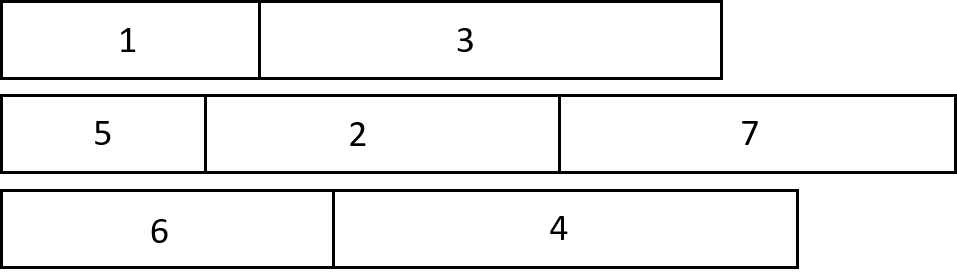
\includegraphics[width=0.5\textwidth]{figure/neighborhood.png}
		\caption{A description of the neighborhood jobs}
		\label{fig:neighborhood}
\end{figure}

In each loop, we randomly swap the neighboring jobs and see if the schedule after the exchange will have a lower tardiness or not. Every swap which has been applied in the recent past will be remembered in a tabu list. If the new swap is in the tabu list, we do not need to swap them again. However, the swap will only be remembered in the tabu list in a limited time. Since the tabu list has a maximum size, when the numbers of swaps exceed its maximum size, the previous swap will be forgotten. The algorithm stops when there are a certain number of consecutive iterations having no improvement.

The overall algorithm process is illustrated in Figure \ref{fig:alg_flow}.
\begin{figure}
		\centering
		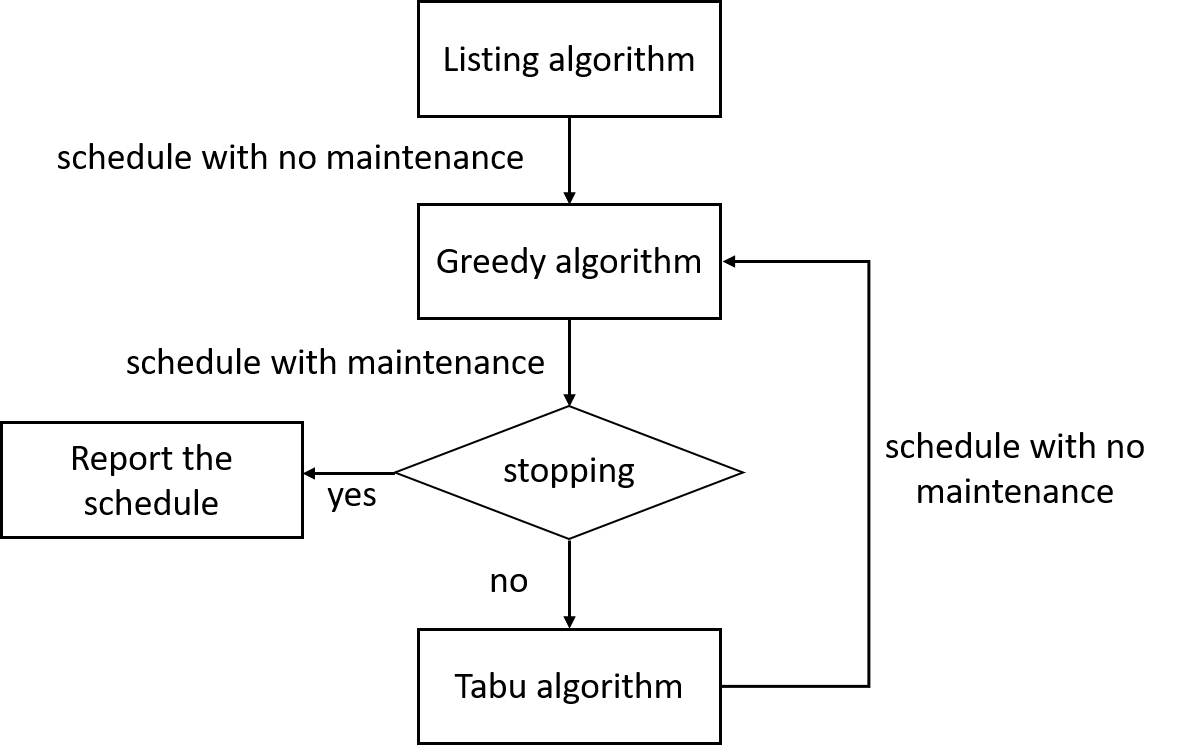
\includegraphics[height=0.4\textwidth]{figure/alg_flow.png}
		\caption{The overall algorithm process}
		\label{fig:alg_flow}
\end{figure}

We conduct extensive numerical studies to observe the performance of our proposed algorithm. For each machine, we set the production rate $A_i$ and the lower bound of yield rate $L_i$ as a fixed number, and set the yield declining rate $B_i$ and the initial yield rate $r_{i,0}$ as a number which are randomly distributed in a certain interval. Each job has a certain demand quantity $Q_j$ and due time $D_j$, which are also randomly distributed in a certain interval. We generate 20 instances for the study. All instances are computed with Gurobi solver and our algorithm. The experiments were performed on a desktop with a 3.6 GHz Intel(R) Core i9-9900K processor and 16 GB RAM. The heuristic algorithm was implemented using python 3.8. And the MIP model was solved using Gurobi 9.1 and implemented through Gurobi python.

To compute the performance of our algorithm, we run the Gurobi model for comparison. Since a MIP model may cost a lot of time to solve the problem, we set the limited time for $1800$ seconds for each problem. Finally, we compare the suboptimal solutions we find in the limited time by Gurobi solver and the suboptimal solutions find by our algorithm.

The average gap is $0.29$ between the algorithm and the solver solution in limited time. However, our algorithm can solve all the problems in $0.1$ second, which is much faster than $1800$ seconds.



%----------------------------------------------------------------------------------------
%	BIBLIOGRAPHY
%----------------------------------------------------------------------------------------

\addcontentsline{toc}{section}{Bibliography}

\bibliographystyle{ormsv080}
\bibliography{MCAC_reference}

\end{document}
